\documentclass[11pt]{article}
\usepackage[brazilian]{babel}
\usepackage[utf8]{inputenc}
\usepackage[T1]{fontenc}
\usepackage[table]{xcolor}
\usepackage{tabularx}
\usepackage[section]{placeins}
%\usepackage[a4paper,margin=1cm,footskip=.5cm]{geometry}
\usepackage{a4wide}
\usepackage{titlesec}
%\usepackage{changepage}
%\setcounter{secnumdepth}{4}
%\setcounter{tocdepth}{4}

\usepackage{hyperref}
\hypersetup{
	colorlinks,
		citecolor=black,
		filecolor=black,
		linkcolor=black,
		urlcolor=black
}

%%%%%%%%%%%%%% SUBSUBSUBSECTION %%%%%%%%%%%%%%
\newenvironment{subs}
	{\adjustwidth{6em}{0pt}}
	{\endadjustwidth}
\titleclass{\subsubsubsection}{straight}[\subsection]

\newcounter{subsubsubsection}[subsubsection]

\renewcommand\thesubsubsubsection{\thesubsubsection.\arabic{subsubsubsection}}
\renewcommand\theparagraph{\thesubsubsubsection.\arabic{paragraph}}
\renewcommand\thesubparagraph{\theparagraph.\arabic{subparagraph}}

\titleformat{\subsubsubsection}
  {\normalfont\normalsize\bfseries}{\thesubsubsubsection}{1em}{}
\titlespacing*{\subsubsubsection}
{0pt}{3.25ex plus 1ex minus .2ex}{1.5ex plus .2ex}

\makeatletter
\renewcommand\paragraph{\@startsection{paragraph}{5}{\z@}%
  {3.25ex \@plus1ex \@minus.2ex}%
  {-1em}%
  {\normalfont\normalsize\bfseries}}
\renewcommand\subparagraph{\@startsection{subparagraph}{6}{\parindent}
  {3.25ex \@plus1ex \@minus .2ex}%
  {-1em}%
  {\normalfont\normalsize\bfseries}}
\def\toclevel@subsubsubsection{4}
\def\toclevel@paragraph{5}
\def\toclevel@paragraph{6}
\def\l@subsubsubsection{\@dottedtocline{4}{7em}{4em}}
\def\l@paragraph{\@dottedtocline{5}{10em}{5em}}
\def\l@subparagraph{\@dottedtocline{6}{14em}{6em}}
\makeatother

\makeatletter
\@addtoreset{subsubsubsection}{section}
\@addtoreset{subsubsubsection}{subsection}
\makeatother

\setcounter{secnumdepth}{6}
\setcounter{tocdepth}{6}
%%%%%%%%%%%%%% SUBSUBSUBSECTION %%%%%%%%%%%%%%
\author{
	Cristiano Bolla Fernandes \\
	Benito Michelon \\
}

\title {Sistemas Embarcados}
\begin{document}
\maketitle
\newpage

\tableofcontents
\newpage

\chapter{\label{chap:intro}Introdução }

\section{\label{sec:secao1}História dos Sistemas de Tempo Real}
lorem ipsum dolor sit $x\leq 2$  amet consetetur sadipscing elitr
sed diam nonumy eirmod Seção~\ref{sec:secao1} tempor invidunt ut
labore et dolore magna aliquyam erat sed diam voluptua at vero eos
et accusam et justo duo dolores et ea rebum stet
clita.~\cite{OLIVEIRAAPL08}

% Um exemplo de fórmula
\begin{equation}\label{eq:eq1}
	\intop_{0}^{\infty}{x^2 + \frac{\pi}{\sum_{i=0}^{n}{\frac{1}{i^2}}}}
\end{equation}

kasd gubergren no sea Equação~\eqref{eq:eq1} takimata sanctus est
lorem ipsum dolor sit amet lorem ipsum dolor sit amet consetetur
sadipscing elitr sed diam nonumy eirmod.~\cite{PICCOLIAPL11}

amet lorem ipsum dolor sit amet consetetur sadipscing elitr sed
diam nonumy eirmod.~\cite{PICCOLIDM08}

\section{\label{sec:secao2}Tempo}
\subsection{Tempo na Execução}
\subsection{Tempo Lógico}
\subsection{Tempo Denso}
\subsection{Tempo Global}
\subsection{Tempo Absoluto}
\subsection{Tempo Relativo}

\section{\label{sec:secao3}Definição de um Sistema de Tempo Real}
\subsection{Aplicações}
\subsection{Problemas clássicos de tempo real}

\section{\label{sec:secao3}Tipos de Sistema de Tempo Real}
\subsection{Críticos}
\subsection{Não críticos}

\section{\label{sec:secao4}Tipos de escalonamentos}
\subsection{Rate monotonic scheduling}
\subsection{Round-Robin}
\subsection{Fixed-Priority}
\subsection{Critical section preemptive scheduling}
\subsection{Static time scheduling}
\subsection{Earliest Deadline First}
\subsection{Cooperative scheduling}


\section{\label{sec:secao5}Avaliação e garantias}
\subsection{Testes}
(Software Engineering: A Practitioner's Approach by Roger S Pressman)
\subsubsection{Teste de tarefas}
\subsubsection{Teste de comportamento}
\subsubsection{Teste intertarefa}
\subsubsection{Teste do sistema}

\subsection{Formalismo em análise de Sistemas de tempo real}
\subsubsection{Metodos de modelagem}
\subsubsection{Uso na indústria}
\subsubsection{Métodos Formais para verificação de sistemas}
\subsubsection{Ferramentas para verificação formal}
lorem ipsum dolor sit amet consetetur sadipscing elitr sed diam nonumy
eirmod tempor invidunt ut labore et dolore magna aliquyam erat sed diam
voluptua at vero eos et accusam et justo duo dolores et ea rebum
stet clita.~\cite{GOLDENBERGAPL02}

\newpage
\section{Sistemas de Tempo Real}
\label{sec:STR}

\subsection{Definição de um Sistema de Tempo Real}
\label{sec:DefSTR}
Um sistema de tempo real, ao contrário do que se costuma pensar, não tem
como objetivo uma execução necessariamente rápida, mas sim, previsível.
Deste tipo de sistema, podemos encontrar duas características fundamentais:

\begin{itemize}
\item Um sistema de tempo real precisa produzir resultados computacionais corretos
(chamados de corretude logica ou funcional).
\item Os resultados computacionalmente corretos obtidos precisam ser concluídos em
um período de tempo pré-definido, caracterizando a previsibilidade na execução da tarefa.
\end{itemize}

Sistemas de tempo real são definidos como sistemas nos quais a corretude nos
resultados de execução de maneira geral são dependentes tanto da corretude
lógica como da previsibilidade do tempo de execução, sendo assim, a previsibilidade
do tempo de execução é, ao menos, tão importante quanto a corretude funcional
nesse tipo de sistemas.~\cite{Li:2003:RCE:829584}

Os sistemas de tempo real são utilizados para atender à tarefas que possuem algum tipo
de restrição temporal em sua execução. Esse tipo de necessidade está muito presente no
dia-a-dia, e são aplicados aos mais diversos tipos de tarefas, desde controladores de
leitores de DVDs, elevadores, freios de carro, controladores de mísseis e até piloto automático
de aeronaves.

\subsection{Tipos de Sistema de Tempo Real}
Como abordado na seção~\ref{sec:DefSTR}, para que um sistemas de tempo real obtenha uma
execução de tarefa correta, é necessário terminar essa execução em um período pré-definido,
chamado de \textit{deadline}. Portanto, é possível afirmar que este tipo de sistema, por possuir
essa restrição temporal, é regido pelos \textit{deadlines} de suas tarefas.

Devido a importância dos \textit{deadlines}, esse tipo de sistema pode ser classificado como
críticos ou não críticos, baseado na tolerância de \textit{deadlines} perdidos, a utilidade
dos resultados computados após a perda do \textit{deadline} e a severidade da penalidade em
perder um prazo de execução.

\subsubsection{Sistemas de Tempo Real Críticos}
Os sistemas de tempo real chamados de críticos são aqueles que possuem uma restrição severa
de prazo na execução de tarefas, ou seja, sua tolerância em perder prazos é muito pequena
ou nenhuma. Em muitos desses sistemas, as informações computadas fora do prazo são consideradas
inúteis, caracterizando uma penalidade grave em perder o prazo de execução.

Um sistema de tempo real crítico é um sistema que precisa executar suas tarefas dentro do prazo
pré-definido com uma tolerância muito próxima de zero. Os prazos devem ser atendidos, ou os resultados
são catastróficos. O custo da perda de prazos na execução possuem um custo muito alto, podendo inclusive
envolver vidas humanas. Os resultados computados após o prazo pré-definido possuem uma utilidade próxima
de zero ou possuem um grande grau de depreciação com a decorrência do tempo após o prazo.~\cite{Li:2003:RCE:829584} \\\\
Alguns exemplos de sistemas de tempo real considerados críticos são:
\begin{itemize}
\item Sistema de navegação de aeronaves.
\item Freios de carro (ABS).
\item Marca-passo.
\item Controladores de mísseis.
\end{itemize}

\subsubsection{Sistemas de Tempo Real Não Críticos}
Os sistemas de tempo real considerados não críticos são aqueles aonde uma perda de prazo
resulta em uma penalidade leve, como uma distorção em uma música sendo lida de um CD, perda
de alguns frames em um vídeo entre outras consequências de baixa criticidade.

Esses sistemas precisam atender seus prazos pré-definidos, porém com um certo grau de flexibilidade.
Os prazos podem possuir diferentes graus de tolerância, prazos balizados com tempo médio e até em avaliação
estatística dos tempos de resposta. Nesse tipo de sistema, apesar da perda de prazos não resultar em uma
falha no sistema, os custos da perda dos mesmos pode se tornar grande, dependendo da proporção em que isso
ocorre.~\cite{Li:2003:RCE:829584} \\\\
Alguns exemplos de sistemas de tempo real considerados não críticos são:
\begin{itemize}
\item Sistema responsável por leitura de DVD.
\item Sistema de som em computadores pessoais.
\item Decodificador de sinal de televisão.
\end{itemize}

\subsection{Validação e Verificação}
Esse tipo de tecnologia precisa possuir a garantia de que o sistema desenvolvido está apto a ser utilizado em produção
e que conseguirá atender à todas as demandas que o serão requisitadas em seu ambiente final de uso.

Segundo Kopetz~\cite{Kopetz:1997:RSD:523911}, até 50\% dos custos de desenvolvimento de um sistema de tempo real, é aplicado
para garantir que o sistema atende completamente à seu propósito. Em aplicações de alta criticidade que necessitam ser certificadas,
essa porcentagem se torna ainda maior.

Para que seja possível garantir essas restrições, dois conceitos são amplamente aplicados,
\textit{verificação}  e \textit{validação}.

A validação atua na avaliação da consistência entre o modelo informal das intenções do usuário e
o comportamento do sistema sendo testado, enquanto a verificação consiste em analisar a consistência
entre a especificação formal criada e o próprio sistema em teste. Enquanto a verificação pode ser
reduzida a um processo formal, a validação precisa avaliar o comportamento do sistema em relação ao mundo real
aonde é aplicado. O principal método de validação é o teste, enquanto o principal método de verificação é a
análise formal.

\subsubsection{Validação}
A validação do sistema busca garantir que o produto desenvolvido atende às necessidades dos usuários. Um dos processos
mais utilizados para esse tipo de análise chama-se \textit{teste de aceitação do usuário}.

O teste de aceitação do usuário é um dos estágios finais do do projeto. Consiste em colocar o sistema a funcionar em seu ambiente final,
sendo operado por seu usuário final verdadeiro, avaliando suas ações e reações durante a utilização. Esse estágio de teste
não procura encontrar erros cosméticos ou mesmo de quebra de software já que esse tipo de problema deve ser eliminado em
estágios anteriores da qualificação do software.

\subsubsection{Testes Padrão de Sistemas}
Segundo Roger S. Pressman~\cite{pre_2005}, o design de caso de testes para sistemas de tempo real pode ser dividido
em quatro passos:

\begin{enumerate}
\item \textbf{Teste de Tarefas}

No princípio, cada tarefa é testada individualmente com maneiras convencionais de testes estáticos, buscando encontrar
apenas erros de lógica ou sintaxe no programa. É um tipo de teste que não leva em conta, especificamente, as peculiaridades
dos sistemas de tempo real, não considerando, ainda, as restrições temporais impostas ao sistema e suas tarefas.


\item \textbf{Teste de Comportamento}

Utilizando os modelos de sistema desenvolvidos com ferramentas para automação de testes, é possível simular os comportamentos
de um sistema de tempo real e os impactos de eventos externos sobre esses comportamentos.


\item \textbf{Teste Intertarefa}

Partindo do pressuposto de que as tarefas estão livres de erros, sendo isso validado pelo \textit{teste de tarefas}, as mesmas são
testadas adicionando ao cenário as características de restrição temporal impostas ao sistema. Esse tipo de teste visa encontrar
erros de comunicação interprocesso, testando tarefas assíncronas com diferentes taxas e tamanhos de dados.


\item \textbf{Teste do Sistema}

Nesse ponto, software e hardware são integrados e uma larga escala de testes de sistema são feitos para encontrar erros durante
a comunicação entre software e hardware.

\end{enumerate}

\subsubsection{Verificação Formal}
A verificação formal consiste em, utilizando uma base matemática de métodos formais, apresentar uma prova ou
contra-prova da corretude de algoritmos de um sistema descrito em uma dada \textit{especificação formal}, melhor
descrita no capítulo~\ref{sec:MFeSTR}.

Este assunto será mais aprofundado, descrevendo suas técnicas em detalhes na segunda etapa deste trabalho.


\newpage
\section{Proposta}
\subsection{Proposta TCC 1}
\subsubsection{Objetivos}
Como objetivos da primeira etapa do trabalho de conclusão, buscamos, em primeiro lugar,
elevar nosso conhecimento nas áreas de sistemas de tempo real e especialmente
em métodos formais, com suas ferramentas e aplicações. Iremos também ,
baseado no conhecimento de pesquisa feita no decorrer deste trabalho, modelar um sistema
nos diferentes métodos formais de modelagem descritos na seção [CITAR SEÇÃO] para fins de
prova de conceito, possibilitando a avaliação destes com base nessas experiências de implementação,
analisando quais são os seus pontos fortes e fracos e quais ferramentas melhor se adaptam às nossas
necessidades para implementarmos a segunda etapa desse trabalho de conclusão.
\\

\paragraph{Sistema Escolhido}\mbox{} \\\\
No mundo da computação vários problemas são resolvidos sem levar em conta o tempo.
Isto decorre da natureza dos problemas obedecerem a lógica não modal, fazendo com que o
problema seja resolvido sem precisarmos atentar a aspectos temporais. Apesar disso,
existem sistemas aonde o aspecto temporal se faz presente, sistemas reativos são um exemplo disto.

Para a análise preliminar dos métodos formais de modelagem propostos, foi escolhido um problema que
já é conhecido pela literatura, exposto por Abrial, B\"{o}rger e Langmaack~\cite{opac-b1092561},
para que seja possível utilizar como exemplo de problema a ser modelado.

O propósito do \textit{Sistema de Aquecimento de Água} (SAA) é o de garantir o funcionamento,
de forma segura, do aquecedor de água. O aquecedor de água opera em segurança se o nível da água
não exceder o limite de tolerância. Além desta restrição, o tanque do sistema tem também
sua resistência à pressão, que não pode ser maior que um valor estipulado pelo fabricante.

O SAA é composto por uma série de sistemas que são necessários para o aquecimento da água e também
para o monitoramento das condições de operação. A seguir são listados os principais subsistemas:
\begin{itemize}
\item Um tanque para o aquecimento da água.
\item Dispositivo para a medição do nível da água.
\item Uma bomba d'água para o abastecimento do tanque.
\item Um dispositivo para a medição da bomba d'água.
\item Um dispositivo para medir a pressão dentro do tanque.
\item Um sistema de controle para atuar nos dispositivos.
\end{itemize}

Para criação da prova de conceito em relação aos métodos formais de modelagem de sistemas préviamente
mencionada, utilizaremos um destes subsistemas, nos capacitando tanto para a escolha do método quanto
para o conhecimento das linguagens, ferramentas e técnicas utilizadas para essa finalidade de modelagem.

\subsubsection{Cronograma}
\renewcommand{\arraystretch}{1.5}
\definecolor{lightgray}{gray}{0.9}
\rowcolors{2}{white}{lightgray}

\newcolumntype{C}{>{\centering\arraybackslash}X}

\begin{tabularx}{\textwidth}{ | c | C | }
\hline
\textbf{Data} & \multicolumn{1}{c|}{\textbf{Evento}} \\
\hline
xx.xx.2014 & Modelagem formal do sistema utilizando Statecharts \\
xx.xx.2014 & Modelagem formal do sistema utilizando Alloy \\
xx.xx.2014 & Modelagem formal do sistema utilizando CSP \\
24.11.2014 & Entrega do Volume Final \\
\hline
\end{tabularx}


\subsubsection{Lista de Atividades}


\subsection{Proposta TCC 2}
\subsubsection{Objetivos}
\subsubsection{Cronograma}
\subsubsection{Lista de Atividades}

\newpage
\section{HellfireOS}
\label{sec:HellfireOS}
O HellfireOS é um sistema operacional de tempo real preemptivo que é parte constituinte
do Hellfire framework (HellfireFW). Projetado para sistemas MPSoC, possui gerenciamento
dinâmico de tarefas que conta com a proteção contra inversão de prioridades e possui as
seguintes políticas de escalonamento:
Rate Monotonic, Round Robin, Earliest Deadline First e Deadline Monotonic.\\
Dentre as bibliotecas que nos interessam consta uma LibC customizada, uma math.h com emulação
de número de ponto flutuante e parte da pilha TCP.\\
Utilizaremos o HellfireOS para controlar os sensores conectados e simulados que iremos utilizar para a nossa
prova de conceito.
\subsection{Arquitetura}
\begin{figure}[H]
	\centering
		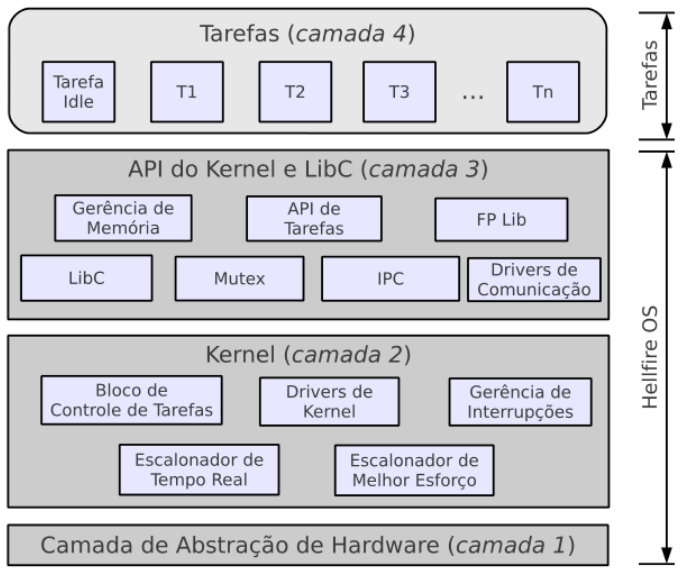
\includegraphics[width=\textwidth,height=\textheight,keepaspectratio]{fig/HellfireArch.png}
	\caption{Arquitetura em alto nível do HellfireOS.}
\end{figure}
%A API do HellfireOS é dividida em 5(cinco) grupos, a saber:
%\begin{itemize}
%	\item Manipulação de Tarefas
%	\item Exclusão Mútua
%	\item Manipulação de Memória
%	\item Comunicação entre processos
%	\item LibC
%\end{itemize}

\newpage
\section{Framework de Integração Que Precisa de um Nome}
\label{sec:Framework}
Descrição das limitações na junção entre COMPaaS e Hellfire e motivação para o desenvolvimento.

\subsection{Arquitetura Proposta}
\subsection{Prova de Conceito}

\newpage
\section{Proposta}
\subsection{Proposta TCC 1}
\subsubsection{Objetivos}
Como objetivos da primeira etapa do trabalho de conclusão, buscamos, em primeiro lugar,
elevar nosso conhecimento nas áreas de sistemas embarcados. Iremos também,
baseado no conhecimento de pesquisa feita no decorrer deste trabalho, criar o ambiente
necessário para efetuar a prova de conceito, obtendo o hardware necessário, e fazendo
as instalações necessárias de sistemas operacionais, host Linux e o HellfireOS, este de forma
virtualizada. Iremos iniciar também as medidas necessárias para suprir a falta de da completude
das camadas de protocolos de rede necessária, implementando uma comunicação através de memória
compartilhada entre os dois sistemas e, inclusive, uma deamon para interfacear o espaço de memória
compartilhada no host Linux e a rede.

\subsubsection{Cronograma}
\renewcommand{\arraystretch}{1.5}
\definecolor{lightgray}{gray}{0.9}
\rowcolors{2}{white}{lightgray}

\newcolumntype{C}{>{\centering\arraybackslash}X}

\begin{tabularx}{\textwidth}{ | c | C | }
\hline
\textbf{Data} & \multicolumn{1}{c|}{\textbf{Evento}} \\
\hline
22.04.2015 & Criação do ambiente da Cubieboard com o host Linux. \\
04.04.2015 & Preparação do ambiente com o suporte e configurações de virtualização necessárias. \\
20.05.2015 & Instalação do HellfireOS de forma virtualizada rodando sobre o host Linux. \\
21.05.2015 & Início da implementação da comunicação entre host e HellfireOS através de memória compartilhada. \\
22.06.2015 & Entrega do Volume Final de TC1. \\
\hline
\end{tabularx}

\subsubsection{Lista de Atividades}
\begin{itemize}
\item Conseguir o hardware necessário para as implementações.
\item Escolha da distribuição adequada para rodar no hardware.
\item Instalação do host no hardware.
\item Pesquisa e configuração do suporte de virtualização no host.
\item Pesquisa e instalação do HellfireOS como sistema virtualizado.
\item Implementação da comunicação entre host e HellfireOS.
\end{itemize}

\subsection{Proposta TCC 2}
\subsubsection{Objetivos}
Nesta etapa iremos finalizar os ajustes necessários do ambiente proposto para teste para então
implementar a integração da plataforma COMPaaS com o sistema HellfireOS,
descritos nas seções~\ref{sec:COMPaaS} e~\ref{sec:HellfireOS} respectivamente, com a criação
do \textit{Hellfire and COMPaaS Integration Layer} (HAC), descrito na seção~\ref{sec:HAC},
objetivando a criação de uma solução completa, desde o sistema operacional embarcado
responsável pela gerência de múltiplos sensores, até a plataforma de IoT, possibilitando
um uso de funcionalidade robusta e simples do HellfireOS na criação e aplicação de
equipamentos integráveis no conceito de \textit{Internet of Things}.
Para prova e testes desta integração, será criado um simulador de sensor da área médica,
baseada em estudos efetuados nesta segunda etapa do trabalho, possibilitando um teste
da integração de forma completa, passando por todos os níveis descritos nas arquiteturas
tanto da plataforma COMPaaS como no HellfireOS nas seções anteriores.

\subsubsection{Cronograma}
\renewcommand{\arraystretch}{1.5}
\definecolor{lightgray}{gray}{0.9}
\rowcolors{2}{white}{lightgray}

\newcolumntype{C}{>{\centering\arraybackslash}X}

\begin{tabularx}{\textwidth}{ | c | C | }
\hline
\textbf{Data} & \multicolumn{1}{c|}{\textbf{Evento}} \\
\hline
07.08.2015 & Implementação da comunicação entre host e HellfireOS através de memória compartilhada. \\
21.08.2015 & Criação da daemon para interfacear a memória compartilhada do host e a rede.  \\
09.10.2015 & Término do desenvolvimento do HAC Integration Layer no HellfireOS. \\
06.11.2015 & Criação do simulador de sensor para prova de conceito da integração. \\
13.11.2015 & Teste completo da implementação. \\
22.11.2015 & Entrega do Volume Final. \\
09.12.2015 & Apresentação do Trabalho. \\
\hline
\end{tabularx}

\subsubsection{Lista de Atividades}
\begin{itemize}
\item Testes para prova da implementação da comunicação entre host e HellfireOS.
\item Definição do funcionamento da daemon proposta.
\item Testes da implementação da daemon de comunicação entre memória compartilhada e rede.
\item Testes do funcionamento da implementação do HAC Integration Layer.
\item Definição das funcionalidades do sensor a ser simulado.
\item Teste para prova da implementação da integração.
\end{itemize}


\newpage

\bibliographystyle{ieeetr}
\bibliography{bibliografia}
\end{document}
